% ============================================================
%  Preparatório OBI — Programação Dinâmica
%  Grupo: GEMA
%  Compilar: pdflatex aula_dp.tex  (rodar 2x)
% ============================================================
\documentclass[aspectratio=169,10pt]{beamer}

\usetheme{Madrid}
\usecolortheme{default}

% ── Pacotes ─────────────────────────────────────────────────
\usepackage[utf8]{inputenc}
\usepackage[T1]{fontenc}
\usepackage[english]{babel}
\usepackage{graphicx}
\usepackage{listings}
\usepackage{xcolor}
\usepackage{tikz}
\usepackage{amsmath}
\usepackage{amssymb}
\usepackage{tcolorbox}
\usepackage{array}
\usepackage{booktabs}
\usepackage{adjustbox}
\usepackage{colortbl}
\tcbuselibrary{skins,breakable,listings}
\usetikzlibrary{arrows.meta,shapes,positioning,fit,calc,
                decorations.pathreplacing,backgrounds,matrix}

% ── Margens ─────────────────────────────────────────────────
\setbeamersize{text margin left=4mm,text margin right=4mm}
\setlength{\leftmargini}{1.0em}
\setlength{\leftmarginii}{0.9em}

% ── Paleta de Cores ─────────────────────────────────────────
\definecolor{gemaBlue}    {RGB}{13,   43,  90}
\definecolor{gemaCyan}    {RGB}{0,   170, 210}
\definecolor{gemaRed}     {RGB}{190,  30,  30}
\definecolor{gemaOrange}  {RGB}{220, 110,   0}
\definecolor{gemaGreen}   {RGB}{30,  150,  70}
\definecolor{gemaPurple}  {RGB}{100,   0, 160}
\definecolor{dpBlue}      {RGB}{20,   80, 180}
\definecolor{dpTeal}      {RGB}{0,   140, 130}
\definecolor{dpGold}      {RGB}{180, 140,   0}
\definecolor{codeBack}    {RGB}{22,   27,  34}
\definecolor{codeGreen}   {RGB}{80,  200, 120}
\definecolor{codeBlue}    {RGB}{121, 192, 255}
\definecolor{codeYellow}  {RGB}{255, 210,  70}
\definecolor{codeOrange}  {RGB}{255, 160,  60}
\definecolor{alertYellow} {RGB}{255, 243, 176}
\definecolor{alertBorder} {RGB}{140, 100,   0}
\definecolor{cellHigh}    {RGB}{200, 230, 255}
\definecolor{cellBase}    {RGB}{240, 248, 255}
\definecolor{cellFill}    {RGB}{30,  120, 200}
\definecolor{cellTrue}    {RGB}{180, 230, 180}
\definecolor{cellFalse}   {RGB}{255, 200, 200}

% ── Cores Beamer ────────────────────────────────────────────
\setbeamercolor{palette primary}    {bg=gemaBlue,  fg=white}
\setbeamercolor{palette secondary}  {bg=gemaBlue!85,fg=white}
\setbeamercolor{palette tertiary}   {bg=gemaBlue!65,fg=white}
\setbeamercolor{palette quaternary} {bg=gemaBlue,  fg=white}
\setbeamercolor{structure}          {fg=gemaBlue}
\setbeamercolor{frametitle}         {fg=white,bg=gemaBlue}
\setbeamercolor{block title}        {fg=white,bg=gemaBlue}
\setbeamercolor{block body}         {fg=black,bg=gemaBlue!7}
\setbeamercolor{block title alerted}{fg=white,bg=gemaRed}
\setbeamercolor{block body alerted} {fg=black,bg=gemaRed!8}
\setbeamercolor{block title example}{fg=white,bg=gemaGreen!75!black}
\setbeamercolor{block body example} {fg=black,bg=gemaGreen!10}
\setbeamercolor{itemize item}       {fg=gemaCyan!70!black}
\setbeamercolor{itemize subitem}    {fg=gemaBlue!60}

\setbeamerfont{frametitle}{size=\large,series=\bfseries}
\setbeamertemplate{navigation symbols}{}

% ── Rodapé ──────────────────────────────────────────────────
\setbeamertemplate{footline}{%
  \leavevmode\hbox{%
    \begin{beamercolorbox}[wd=.33\paperwidth,ht=2.8ex,dp=1.2ex,center]{palette secondary}
      \tiny GEMA
    \end{beamercolorbox}%
    \begin{beamercolorbox}[wd=.34\paperwidth,ht=2.8ex,dp=1.2ex,center]{palette primary}
      \tiny Programação Dinâmica
    \end{beamercolorbox}%
    \begin{beamercolorbox}[wd=.33\paperwidth,ht=2.8ex,dp=1.2ex,right]{palette secondary}
      \tiny \insertframenumber/\inserttotalframenumber\hspace{2mm}
    \end{beamercolorbox}%
  }%
}

% ── Estilos de Código C++ ───────────────────────────────────
\lstdefinestyle{cppstyle}{
  language=C++,
  backgroundcolor=\color{codeBack},
  basicstyle=\ttfamily\scriptsize\color{white},
  keywordstyle=\color{codeBlue}\bfseries,
  stringstyle=\color{codeOrange},
  commentstyle=\color{codeGreen}\itshape,
  numberstyle=\tiny\color{gray!60},
  identifierstyle=\color{white},
  morekeywords={vector,pair,sort,auto,bool,long,string,
                int64\_t,size\_t,ll,INF},
  emph={push\_back,push,pop,top,front,empty,size,
        cout,cin,endl,min,max,fill,memset},
  emphstyle=\color{codeYellow}\bfseries,
  numbers=left, numbersep=5pt,
  frame=none, tabsize=4,
  showstringspaces=false,
  breaklines=true, columns=flexible, keepspaces=true,
  xleftmargin=10pt, aboveskip=0pt, belowskip=0pt,
}
\lstdefinestyle{cppsmall}{
  style=cppstyle,
  basicstyle=\ttfamily\tiny\color{white},
  numberstyle=\tiny\color{gray!50},
  numbersep=3pt, xleftmargin=7pt, lineskip=-0.5pt,
}

% ── Caixas tcolorbox ────────────────────────────────────────
\tcbset{
  before skip=1pt, after skip=1pt, boxsep=0pt,
  caixaBase/.style={enhanced,arc=4pt,boxrule=0.8pt,
    left=3pt,right=3pt,top=2pt,bottom=2pt,
    fonttitle=\bfseries\footnotesize},
  caixaAzul/.style={caixaBase,
    colback=gemaBlue!6,colframe=gemaBlue},
  caixaDP/.style={caixaBase,
    colback=dpBlue!8,colframe=dpBlue,
    fonttitle=\bfseries\footnotesize\color{dpBlue!70!black}},
  caixaTeal/.style={caixaBase,
    colback=dpTeal!8,colframe=dpTeal,
    fonttitle=\bfseries\footnotesize\color{dpTeal!70!black}},
  caixaVerde/.style={caixaBase,
    colback=gemaGreen!8,colframe=gemaGreen!60!black,
    fonttitle=\bfseries\footnotesize\color{gemaGreen!35!black}},
  caixaVermelho/.style={caixaBase,
    colback=gemaRed!8,colframe=gemaRed,
    fonttitle=\bfseries\footnotesize\color{gemaRed!80!black}},
  caixaLaranja/.style={caixaBase,
    colback=gemaOrange!8,colframe=gemaOrange,
    fonttitle=\bfseries\footnotesize\color{gemaOrange!80!black}},
  caixaDourada/.style={caixaBase,
    colback=dpGold!10,colframe=dpGold,
    fonttitle=\bfseries\footnotesize\color{dpGold!70!black}},
  caixaRoxa/.style={caixaBase,
    colback=gemaPurple!8,colframe=gemaPurple!70,
    fonttitle=\bfseries\footnotesize\color{gemaPurple!70!black}},
  caixaAmarelo/.style={caixaBase,
    colback=alertYellow,colframe=alertBorder,
    fonttitle=\bfseries\footnotesize\color{alertBorder}},
  caixaCodigo/.style={enhanced,arc=4pt,boxrule=0.8pt,
    colback=codeBack,colframe=gemaCyan!45,
    left=1pt,right=1pt,top=1pt,bottom=1pt},
}

% ── Comando para célula de tabela DP ────────────────────────
\newcommand{\cDP}[1]{%
  \cellcolor{cellBase}\footnotesize #1}
\newcommand{\cDPh}[1]{%
  \cellcolor{cellHigh}\footnotesize\bfseries #1}
\newcommand{\cDPf}[1]{%
  \cellcolor{cellFill}\footnotesize\bfseries\color{white} #1}
\newcommand{\cDPT}[1]{%
  \cellcolor{cellTrue}\footnotesize\bfseries #1}
\newcommand{\cDPF}[1]{%
  \cellcolor{cellFalse}\footnotesize #1}

% ── Metadados ───────────────────────────────────────────────
\title[DP --- Programação Dinâmica]{Programação Dinâmica}
\subtitle{Preparatorio OBI --- Do Recursivo ao Otimo}
\author[GEMA]{Grupo de Extensao em Maratonas de Programação}
\institute{GEMA}
\date{2025}

% ============================================================
\begin{document}
% ============================================================

% ── SLIDE DE TÍTULO ─────────────────────────────────────────
{
\setbeamertemplate{footline}{}
\begin{frame}[noframenumbering]
  \begin{columns}[c]
    \column{0.62\textwidth}
      \vspace{0.15cm}
      {\fontsize{22}{26}\selectfont\bfseries\color{gemaBlue}
        Programação Dinâmica\par}
      \vspace{0.08cm}
      {\fontsize{13}{16}\selectfont\color{dpTeal}\bfseries
        Dynamic Programming\par}
      \vspace{0.14cm}
      {\large\color{gemaCyan}
        Preparatório OBI --- Ala 05\par}
      \vspace{0.30cm}
    \column{0.36\textwidth}
      \centering
      
\includegraphics[width=0.50\linewidth]{logo.png}\\[0.28cm]
      
\includegraphics[width=0.50\linewidth]{logo_obi.png}
  \end{columns}
\end{frame}
}

% ── AGENDA ──────────────────────────────────────────────────
\begin{frame}{Agenda}
  \begin{columns}[t]
    \column{0.48\textwidth}
      \begin{block}{Fundamentos}
        \begin{enumerate}\footnotesize
          \item Motivação: o problema da recursão
          \item O que e Programação Dinâmica?
          \item Subproblemas sobrepostos
          \item Os quatro pilares: estado, transição,
                base, ordem
          \item Memoization vs Tabulação
        \end{enumerate}
      \end{block}
      \vspace{0.12cm}
      \begin{block}{Exemplos Classicos}
        \begin{enumerate}\setcounter{enumi}{5}\footnotesize
          \item Fibonacci
          \item Mochila 0/1 (Knapsack)
          \item Subset Sum
        \end{enumerate}
      \end{block}
    \column{0.48\textwidth}
      \begin{block}{Pratica e Competição}
        \begin{enumerate}\setcounter{enumi}{8}\footnotesize
          \item Complexidade: espaçoe tempo
          \item Como pensar em DP (passo a passo)
          \item Como identificar na OBI
          \item Erros comuns
          \item Problemas para praticar
        \end{enumerate}
      \end{block}
      \vspace{0.12cm}
      \begin{tcolorbox}[caixaDP,title={Ideia central}]
        \footnotesize
        DP = \textbf{recursão} + \textbf{Memorização}.\\
        Resolvemos cada subproblema \textbf{uma unica vez}
        e reutilizamos a resposta.
      \end{tcolorbox}
  \end{columns}
\end{frame}

% ============================================================
%  PARTE 1 — FUNDAMENTOS
% ============================================================
{
\setbeamertemplate{footline}{}
\begin{frame}[noframenumbering]
  \centering\vspace{1.0cm}
  {\fontsize{36}{44}\selectfont\bfseries\color{gemaBlue} 1}\par
  \vspace{0.22cm}
  {\Large\color{dpTeal}\bfseries Fundamentos}\par
  \vspace{0.14cm}
  {\color{gray}\small Motivação $\cdot$ Conceitos $\cdot$ Pilares $\cdot$ Abordagens}
\end{frame}
}

% ── MOTIVAÇÃO: O PROBLEMA DA RECURSÃO ───────────────────────
\begin{frame}{Motivação --- O Problema da recursão Ingenua}
  \begin{columns}[c]
    \column{0.46\textwidth}
      \begin{tcolorbox}[caixaVermelho,title={Fibonacci Recursivo}]
        \footnotesize
        \texttt{fib(5) = fib(4) + fib(3)}\\
        \texttt{fib(4) = fib(3) + fib(2)}\\
        \texttt{fib(3) = fib(2) + fib(1)}\\[3pt]
        \textbf{fib(3) e calculado 2 vezes!}\\
        \textbf{fib(2) e calculado 3 vezes!}\\[3pt]
        Complexidade: \textbf{O($2^n$)} \textcolor{gemaRed}{\texttimes}
      \end{tcolorbox}
      \vspace{0.10cm}
      \begin{tcolorbox}[caixaAmarelo,title={O problema central}]
        \footnotesize
        A recursão \textbf{recalcula} subproblemas
        que já foram resolvidos antes.\\[3pt]
        Para $n=40$: $\approx 10^9$ chamadas.\\
        Para $n=60$: $\approx 10^{18}$ chamadas.\\[3pt]
        \textbf{Solução:} guardar o resultado!
      \end{tcolorbox}
    \column{0.52\textwidth}
      \centering
      % Arvore de chamadas fib(5)
      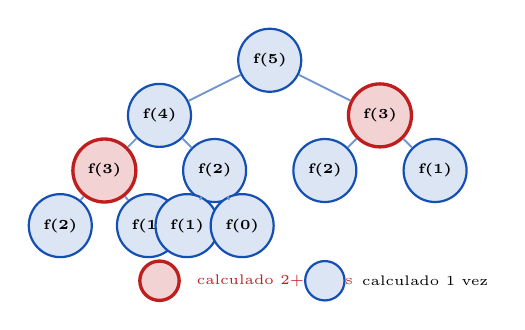
\begin{tikzpicture}[scale=0.70,
        no/.style={circle,draw=dpBlue,fill=dpBlue!15,
                   minimum size=8mm,font=\bfseries\tiny,line width=0.8pt},
        dup/.style={circle,draw=gemaRed,fill=gemaRed!20,
                    minimum size=8mm,font=\bfseries\tiny,line width=1.2pt},
        ed/.style={draw=dpBlue!60,line width=0.7pt}]

        \node[no] (f5) at (4.0,4.2) {f(5)};
        \node[no] (f4) at (2.0,3.2) {f(4)};
        \node[dup](f3a) at (6.0,3.2) {f(3)};
        \node[dup](f3b) at (1.0,2.2) {f(3)};
        \node[no] (f2a) at (3.0,2.2) {f(2)};
        \node[no] (f2b) at (5.0,2.2) {f(2)};
        \node[no] (f1a) at (7.0,2.2) {f(1)};
        \node[no] (f2c) at (0.2,1.2) {f(2)};
        \node[no] (f1b) at (1.8,1.2) {f(1)};
        \node[no] (f1c) at (2.5,1.2) {f(1)};
        \node[no] (f0a) at (3.5,1.2) {f(0)};

        \foreach \a/\b in {f5/f4,f5/f3a,f4/f3b,f4/f2a,
                            f3a/f2b,f3a/f1a,f3b/f2c,f3b/f1b,
                            f2a/f1c,f2a/f0a}{
          \draw[ed] (\a)--(\b);
        }

        % Legenda
        \node[dup,minimum size=5mm] at (2.0,0.2){};
        \node[font=\tiny,right] at (2.5,0.2){\textcolor{gemaRed}{calculado 2+ vezes}};
        \node[no,minimum size=5mm] at (5.0,0.2){};
        \node[font=\tiny,right] at (5.5,0.2){calculado 1 vez};
      \end{tikzpicture}
  \end{columns}
\end{frame}

% ── O QUE É DP ──────────────────────────────────────────────
\begin{frame}{O que e Programação Dinâmica?}
  \begin{columns}[c]
    \column{0.50\textwidth}
      \begin{tcolorbox}[caixaDP,title={Definição}]
        \small
        Programação Dinâmica e uma tecnica de
        \textbf{otimização} que resolve problemas
        dividindo-os em \textbf{subproblemas menores}
        e \textbf{armazenando} os resultados para
        evitar recomputação.
      \end{tcolorbox}
      \vspace{0.10cm}
      \begin{tcolorbox}[caixaAzul,title={Dois ingredientes obrigatorios}]
        \begin{enumerate}\footnotesize
          \item \textbf{Subproblemas sobrepostos:}\\
                o mesmo subproblema aparece multiplas vezes
          \item \textbf{Subestrutura ótima:}\\
                a solução otima contem soluções\\
                ótimas dos subproblemas
        \end{enumerate}
      \end{tcolorbox}
      \vspace{0.10cm}
      \begin{tcolorbox}[caixaAmarelo,title={Resumo em uma linha}]
        \footnotesize
        \textbf{DP = recursão + Memoização}\\
        Resolve cada subproblema \textbf{exatamente uma vez}.
      \end{tcolorbox}
    \column{0.48\textwidth}
      \centering
      % Diagrama comparativo
      \begin{tikzpicture}[scale=0.76]
        \node[font=\bfseries\footnotesize,gemaBlue] at (3.0,4.8)
          {Comparação de abordagens};

        % Forca bruta
        \node[draw=gemaRed!70,fill=gemaRed!8,rounded corners=4pt,
              minimum width=2.5cm,minimum height=1.4cm] at (1.0,3.4){};
        \node[font=\bfseries\tiny,gemaRed] at (1.0,3.9){Forca Bruta};
        \node[font=\tiny,align=center] at (1.0,3.3){Recalcula\\ tudo};
        \node[font=\tiny,gemaRed] at (1.0,2.8){O($2^n$)};

        % DP
        \node[draw=dpBlue,fill=dpBlue!10,rounded corners=4pt,
              minimum width=2.5cm,minimum height=1.4cm,line width=1.2pt]
              at (3.0,3.4){};
        \node[font=\bfseries\tiny,dpBlue] at (3.0,3.9){\textbf{Prog. Dinamica}};
        \node[font=\tiny,align=center] at (3.0,3.3){Resolve 1x\\ reutiliza};
        \node[font=\tiny,dpBlue,bfseries] at (3.0,2.8){O(n$\cdot$k)};

        % Guloso
        \node[draw=gemaGreen!60!black,fill=gemaGreen!8,rounded corners=4pt,
              minimum width=2.5cm,minimum height=1.4cm] at (5.0,3.4){};
        \node[font=\bfseries\tiny,gemaGreen!60!black] at (5.0,3.9){Guloso};
        \node[font=\tiny,align=center] at (5.0,3.3){Escolha\\ local};
        \node[font=\tiny,gemaGreen!60!black] at (5.0,2.8){O(n log n)};

        % Flechas e labels
        \draw[-{Stealth},gray!50,thin](1.0,2.5)--(1.0,2.0);
        \node[font=\tiny,gray,align=center] at (1.0,1.7){sem \\ garantia};
        \draw[-{Stealth},dpBlue,line width=1pt](3.0,2.5)--(3.0,2.0);
        \node[font=\bfseries\tiny,dpBlue,align=center] at (3.0,1.7){otimo \\ garantido};
        \draw[-{Stealth},gray!50,thin](5.0,2.5)--(5.0,2.0);
        \node[font=\tiny,gray,align=center] at (5.0,1.7){se tiver\\ propriedade};

        \node[font=\tiny,gray,align=center] at (3.0,0.8)
          {DP: o melhor dos dois mundos};
      \end{tikzpicture}
  \end{columns}
\end{frame}

% ── OS 4 PILARES ────────────────────────────────────────────
\begin{frame}{Os Quatro Pilares da Programação Dinâmica}
  \begin{columns}[t]
    \column{0.48\textwidth}
      \begin{tcolorbox}[caixaDP,title={1. Estado}]
        \footnotesize
        O que \textbf{precisamos saber} para resolver
        um subproblema.\\[3pt]
        Geralmente representado como \textbf{dp[i]},
        \textbf{dp[i][j]}, etc.\\[3pt]
        \textit{Exemplo (Fibonacci):}\\
        \texttt{dp[i]} = i-ésimo número de Fibonacci.
      \end{tcolorbox}
      \vspace{0.10cm}
      \begin{tcolorbox}[caixaTeal,title={2. Transição (Recorrência)}]
        \footnotesize
        Como \textbf{combinar} estados menores para
        resolver um estado maior.\\[3pt]
        E a \textbf{fórmula recursiva} da DP.\\[3pt]
        \textit{Exemplo:}\\
        \texttt{dp[i] = dp[i-1] + dp[i-2]}
      \end{tcolorbox}
    \column{0.48\textwidth}
      \begin{tcolorbox}[caixaVerde,title={3. Caso Base}]
        \footnotesize
        Subproblemas \textbf{triviais} que conhecemos
        a resposta sem computar.\\[3pt]
        Sem base, a recursão nao termina!\\[3pt]
        \textit{Exemplo:}\\
        \texttt{dp[0] = 0, dp[1] = 1}
      \end{tcolorbox}
      \vspace{0.10cm}
      \begin{tcolorbox}[caixaLaranja,title={4. Ordem de Computação}]
        \footnotesize
        Em qual \textbf{sequência} calcular os estados
        para que as dependências estejam prontas.\\[3pt]
        \textit{Tabulação:} de baixo para cima (bottom-up).\\
        \textit{Memoization:} top-down com cache.
      \end{tcolorbox}
  \end{columns}
\end{frame}

% ── MEMOIZATION VS TABULAÇÃO ────────────────────────────────
\begin{frame}{Memoization vs Tabulação}
  \begin{columns}[t]
    \column{0.48\textwidth}
      \begin{tcolorbox}[caixaDP,title={Memoization (Top-Down)}]
        \footnotesize
        \textbf{Ideia:} use recursão, mas guarde os
        resultados num array/mapa.\\[3pt]
        \textbf{Vantagens:}
        \begin{itemize}\footnotesize
          \item Fácil de implementar (modifica recursão)
          \item Calcula apenas o que precisa
          \item Intuitivo (pensa recursivo)
        \end{itemize}
        \textbf{Desvantagens:}
        \begin{itemize}\footnotesize
          \item Overhead de chamadas recursivas
          \item Pode causar stack overflow (n grande)
        \end{itemize}
      \end{tcolorbox}
    \column{0.48\textwidth}
      \begin{tcolorbox}[caixaTeal,title={Tabulação (Bottom-Up)}]
        \footnotesize
        \textbf{Ideia:} preencha uma tabela iterativamente,
        dos casos baseatéa resposta.\\[3pt]
        \textbf{Vantagens:}
        \begin{itemize}\footnotesize
          \item Sem overhead de recursão
          \item Mais rápido na pratica
          \item Sem risco de stack overflow
        \end{itemize}
        \textbf{Desvantagens:}
        \begin{itemize}\footnotesize
          \item Exige pensar na ordem de cálculo
          \item Pode calcular estados desnecessarios
        \end{itemize}
      \end{tcolorbox}
  \end{columns}
  \vspace{0.10cm}
  \begin{tcolorbox}[caixaAmarelo,title={Qual usar na OBI?}]
    \footnotesize
    \textbf{Ambas são aceitas.}
    Em competição, prefira \textbf{tabulação} (mais rapida, sem stack overflow).
    Memoization é otima para \textbf{prototipar} a solução rapidamente.
    Muitas soluções de maratona usam tabulação com um loop simples.
  \end{tcolorbox}
\end{frame}

% ============================================================
%  PARTE 2 — EXEMPLOS CLÁSSICOS
% ============================================================
{
\setbeamertemplate{footline}{}
\begin{frame}[noframenumbering]
  \centering\vspace{1.0cm}
  {\fontsize{36}{44}\selectfont\bfseries\color{gemaBlue} 2}\par
  \vspace{0.22cm}
  {\Large\color{dpTeal}\bfseries Exemplos Classicos}\par
  \vspace{0.14cm}
  {\color{gray}\small Fibonacci $\cdot$ Mochila 0/1 $\cdot$ Subset Sum}
\end{frame}
}

% ── FIBONACCI: ABORDAGENS ───────────────────────────────────
\begin{frame}{Fibonacci --- As Tres Abordagens}
  \centering
  \begin{adjustbox}{max totalsize={0.97\textwidth}{0.80\textheight},center}
  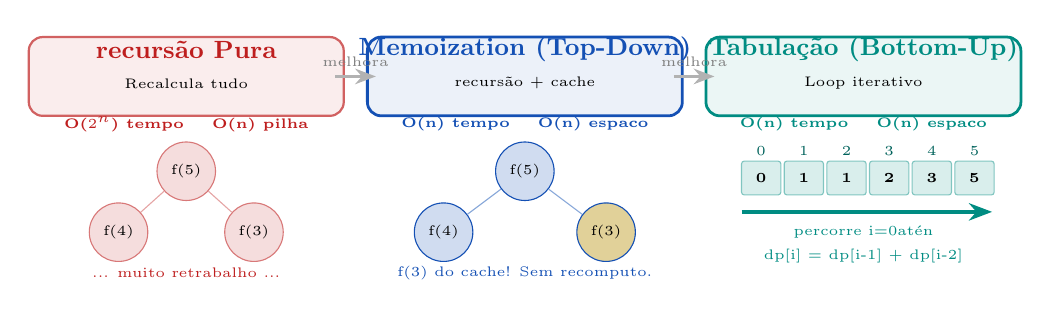
\begin{tikzpicture}[scale=0.86]

    % ── recursão ─────────────────────────────────────────
    \node[draw=gemaRed!70,fill=gemaRed!8,rounded corners=5pt,
          minimum width=4.0cm,minimum height=1.0cm,line width=0.8pt]
          at (2.0,5.2){};
    \node[font=\bfseries\small,gemaRed] at (2.0,5.6){recursão Pura};
    \node[font=\tiny,align=center] at (2.0,5.1){Recalcula tudo};
    \node[font=\bfseries\tiny,gemaRed,below] at (2.0,4.75){O($2^n$) tempo \quad O(n) pilha};

    % arvore recursiva (simplificada)
    \node[circle,draw=gemaRed!60,fill=gemaRed!15,
          minimum size=7mm,font=\tiny] (r5) at (2.0,3.8){f(5)};
    \node[circle,draw=gemaRed!60,fill=gemaRed!15,
          minimum size=6mm,font=\tiny] (r4) at (1.0,2.9){f(4)};
    \node[circle,draw=gemaRed!60,fill=gemaRed!15,
          minimum size=6mm,font=\tiny] (r3) at (3.0,2.9){f(3)};
    \foreach \a/\b in {r5/r4,r5/r3}{\draw[gemaRed!40,thin](\a)--(\b);}
    \node[font=\tiny,gemaRed] at (2.0,2.3){... muito retrabalho ...};

    % ── MEMOIZATION ──────────────────────────────────────
    \node[draw=dpBlue,fill=dpBlue!8,rounded corners=5pt,
          minimum width=4.0cm,minimum height=1.0cm,line width=1pt]
          at (7.0,5.2){};
    \node[font=\bfseries\small,dpBlue] at (7.0,5.6){Memoization (Top-Down)};
    \node[font=\tiny,align=center] at (7.0,5.1){recursão + cache};
    \node[font=\bfseries\tiny,dpBlue,below] at (7.0,4.75){O(n) tempo \quad O(n) espaco};

    % arvore com cache
    \node[circle,draw=dpBlue,fill=dpBlue!20,
          minimum size=7mm,font=\tiny] (m5) at (7.0,3.8){f(5)};
    \node[circle,draw=dpBlue,fill=dpBlue!20,
          minimum size=6mm,font=\tiny] (m4) at (5.8,2.9){f(4)};
    \node[circle,draw=dpBlue,fill=dpGold!40,
          minimum size=6mm,font=\tiny] (m3) at (8.2,2.9){f(3)};
    \foreach \a/\b in {m5/m4,m5/m3}{\draw[dpBlue!50,thin](\a)--(\b);}
    \node[font=\tiny,dpBlue] at (7.0,2.3){f(3) do cache! Sem recomputo.};

    % ── TABULAção ────────────────────────────────────────
    \node[draw=dpTeal,fill=dpTeal!8,rounded corners=5pt,
          minimum width=4.0cm,minimum height=1.0cm,line width=1pt]
          at (12.0,5.2){};
    \node[font=\bfseries\small,dpTeal] at (12.0,5.6){Tabulação (Bottom-Up)};
    \node[font=\tiny,align=center] at (12.0,5.1){Loop iterativo};
    \node[font=\bfseries\tiny,dpTeal,below] at (12.0,4.75){O(n) tempo \quad O(n) espaco};

    % Tabela preenchida
    \foreach \i/\v in {0/0,1/1,2/1,3/2,4/3,5/5}{
      \pgfmathsetmacro{\xpos}{10.2 + \i*0.63}
      \draw[dpTeal!50,fill=dpTeal!15,rounded corners=1pt]
        (\xpos,3.45) rectangle (\xpos+0.58,3.95);
      \node[font=\tiny,dpTeal!70!black] at (\xpos+0.29,4.1){\i};
      \node[font=\bfseries\tiny] at (\xpos+0.29,3.7){\v};
    }
    \draw[-{Stealth},dpTeal,line width=1.2pt](10.2,3.2)--(13.9,3.2);
    \node[font=\tiny,dpTeal] at (12.0,2.9){percorre i=0atén};
    \node[font=\tiny,dpTeal] at (12.0,2.55){dp[i] = dp[i-1] + dp[i-2]};

    % Setas entre abordagens
    \draw[-{Stealth},gray!60,line width=1pt](4.2,5.2)--(4.8,5.2);
    \node[font=\tiny,gray,above] at (4.5,5.2){melhora};
    \draw[-{Stealth},gray!60,line width=1pt](9.2,5.2)--(9.8,5.2);
    \node[font=\tiny,gray,above] at (9.5,5.2){melhora};

  \end{tikzpicture}
  \end{adjustbox}
\end{frame}

% % ── FIBONACCI: CÓDIGO ───────────────────────────────────────
% \begin{frame}[fragile,shrink=3]{Fibonacci --- Codigo C++: Tres Abordagens}
%   \begin{columns}[t]
%     \column{0.49\textwidth}
%       \begin{tcolorbox}[caixaVermelho,title={recursão Pura (EVITAR)}]
%         \begin{tcolorbox}[caixaCodigo]
%           \begin{lstlisting}[style=cppsmall]
% // O(2^n) -- MUITO LENTO
% long long fib(int n){
%     if(n <= 1) return n;
%     return fib(n-1) + fib(n-2);
% }
%           \end{lstlisting}
%         \end{tcolorbox}
%       \end{tcolorbox}
%       \vspace{0.06cm}
%       \begin{tcolorbox}[caixaDP,title={Memoization (Top-Down)}]
%         \begin{tcolorbox}[caixaCodigo]
%           \begin{lstlisting}[style=cppsmall]
% // O(n) -- com cache
% long long memo[100];
% bool calc[100];

% long long fib(int n){
%     if(n <= 1) return n;
%     if(calc[n]) return memo[n];
%     calc[n] = true;
%     return memo[n] = fib(n-1)+fib(n-2);
% }
% // Inicializar: memset(calc,0,sizeof calc)
%           \end{lstlisting}
%         \end{tcolorbox}
%       \end{tcolorbox}
%     \column{0.49\textwidth}
%       \begin{tcolorbox}[caixaTeal,title={Tabulação (Bottom-Up) --- PREFERIR}]
%         \begin{tcolorbox}[caixaCodigo]
%           \begin{lstlisting}[style=cppstyle]
% #include <bits/stdc++.h>
% using namespace std;
% typedef long long ll;

% int main(){
%     int n; cin >> n;
%     vector<ll> dp(n+1);

%     // Casos base
%     dp[0] = 0;
%     dp[1] = 1;

%     // Transição: dp[i] = dp[i-1] + dp[i-2]
%     for(int i = 2; i <= n; i++)
%         dp[i] = dp[i-1] + dp[i-2];

%     cout << dp[n] << "\n";
%     return 0;
% }
%           \end{lstlisting}
%         \end{tcolorbox}
%       \end{tcolorbox}
%       \begin{tcolorbox}[caixaAzul,title={Otimização de espaco}]
%         \footnotesize
%         Fibonacci so precisa dos 2 anteriores:\\
%         O(1) de espaçocom duas variaveis!\\
%         \texttt{a, b = b, a+b}
%       \end{tcolorbox}
%   \end{columns}
% \end{frame}

% ── MOCHILA 0/1: ENUNCIADO E ESTADO ────────────────────────
\begin{frame}{Mochila 0/1 (Knapsack) --- Problema e Modelagem}
  \begin{columns}[c]
    \column{0.48\textwidth}
      \begin{tcolorbox}[caixaAzul,title={Enunciado}]
        \small
        Dados $n$ itens, cada um com \textbf{peso} $w_i$
        e \textbf{valor} $v_i$, e uma mochila de
        capacidade $W$, escolha itens para
        \textbf{maximizar o valor total}
        sem exceder $W$.\\[4pt]
        \textbf{Restrição:} cada item ou vai inteiro
        (1) ou nao vai (0) --- sem fracionr.
      \end{tcolorbox}
      \vspace{0.10cm}
      \begin{tcolorbox}[caixaDP,title={Estado}]
        \footnotesize
        \texttt{dp[i][j]} = valor maximo usando
        os \textbf{primeiros i itens} com
        \textbf{capacidade j}.
      \end{tcolorbox}
      \vspace{0.10cm}
      \begin{tcolorbox}[caixaTeal,title={Transição}]
        \footnotesize
        Para cada item $i$ com peso $w_i$ e valor $v_i$:\\[3pt]
        \textbf{Nao pega:} \texttt{dp[i][j] = dp[i-1][j]}\\
        \textbf{Pega} (se $j \geq w_i$):\\
        \texttt{dp[i][j] = dp[i-1][j-wi] + vi}\\[3pt]
        \texttt{dp[i][j] = max(nao pega, pega)}
      \end{tcolorbox}
    \column{0.50\textwidth}
      \centering
      % Visualização da mochila e itens
      \begin{tikzpicture}[scale=0.78]
        \node[font=\bfseries\footnotesize,gemaBlue] at (3.5,4.8)
          {Exemplo: W=5};

        % Itens
        \node[font=\bfseries\tiny,gemaBlue] at (-0.2,4.2){Itens:};
        \foreach \i/\w/\v/\col/\y in {
          1/2/3/dpBlue/3.7,
          2/3/4/dpTeal/3.1,
          3/2/5/gemaGreen/2.5,
          4/1/2/gemaOrange/1.9}{
          \draw[fill=\col!20,draw=\col!70,rounded corners=2pt,
                minimum width=1.5cm]
            (0.0,\y-0.22) rectangle (1.2,\y+0.22)
            node[midway,font=\tiny,\col!60!black]
              {\textbf{\i}: w=\w, v=\v};
        }

        % Mochila
        \draw[gemaBlue!50,line width=1.5pt,rounded corners=5pt]
          (2.5,1.5) rectangle (4.5,4.5);
        \node[font=\bfseries\tiny,gemaBlue] at (3.5,4.8){Mochila (W=5)};

        % Itens na mochila: 1(w=2)+3(w=2)+4(w=1)=5, valor=10
        \draw[fill=dpBlue!30,draw=dpBlue!70,rounded corners=2pt]
          (2.6,1.6) rectangle (4.4,2.2)
          node[midway,font=\tiny\bfseries,dpBlue!60!black]{Item 4 (w=1, v=2)};
        \draw[fill=gemaGreen!30,draw=gemaGreen!70,rounded corners=2pt]
          (2.6,2.3) rectangle (4.4,3.3)
          node[midway,font=\tiny\bfseries,gemaGreen!60!black]{Item 3 (w=2, v=5)};
        \draw[fill=dpBlue!20,draw=dpBlue!70,rounded corners=2pt]
          (2.6,3.4) rectangle (4.4,4.4)
          node[midway,font=\tiny\bfseries,dpBlue!60!black]{Item 1 (w=2, v=3)};

        \node[font=\bfseries\tiny,gemaGold!70!black] at (3.5,1.2)
          {Valor total: 2+5+3=\textbf{10}};
        \node[font=\tiny,gray] at (3.5,0.85)
          {Peso: 1+2+2=5 = W};
      \end{tikzpicture}
  \end{columns}
\end{frame}

% ── MOCHILA: TABELA PASSO A PASSO ───────────────────────────
\begin{frame}[shrink=3]{Mochila 0/1 --- Tabela DP Passo a Passo}
  \begin{tcolorbox}[caixaAzul,title={Itens: (w=2,v=3), (w=3,v=4), (w=2,v=5) --- Capacidade W=5}]
    \centering\footnotesize
    \setlength{\tabcolsep}{3pt}
    \begin{tabular}{c|cccccc}
      \toprule
      \rowcolor{gemaBlue!15}
      \textbf{dp[i][j]} & \textbf{j=0} & \textbf{j=1} & \textbf{j=2} & \textbf{j=3} & \textbf{j=4} & \textbf{j=5}\\
      \midrule
      \textbf{i=0} (nenhum) & \cDP{0} & \cDP{0} & \cDP{0} & \cDP{0} & \cDP{0} & \cDP{0}\\
      \textbf{i=1} (w=2,v=3) & \cDP{0} & \cDP{0} & \cDPh{3} & \cDPh{3} & \cDPh{3} & \cDPh{3}\\
      \textbf{i=2} (w=3,v=4) & \cDP{0} & \cDP{0} & \cDP{3} & \cDPh{4} & \cDPh{4} & \cDPh{7}\\
      \textbf{i=3} (w=2,v=5) & \cDP{0} & \cDP{0} & \cDPh{5} & \cDPh{5} & \cDPh{8} & \cDPh{9}\\
      \bottomrule
    \end{tabular}
  \end{tcolorbox}
  \vspace{0.08cm}
  \begin{columns}[t]
    \column{0.48\textwidth}
      \begin{tcolorbox}[caixaTeal,title={Como preencher dp[3][5]?}]
        \footnotesize
        Item 3: peso=2, valor=5\\[2pt]
        \textbf{Nao pega:} dp[2][5] = 7\\
        \textbf{Pega:} dp[2][5-2] + 5 = dp[2][3] + 5 = 4+5 = 9\\[2pt]
        dp[3][5] = max(7, 9) = \textbf{9}
      \end{tcolorbox}
    \column{0.48\textwidth}
      \begin{tcolorbox}[caixaVerde,title={Resposta}]
        \footnotesize
        \textbf{dp[n][W]} = valor maximo obtido.\\[2pt]
        No exemplo: dp[3][5] = \textbf{9}\\[2pt]
        (pegar itens 2 e 3: w=3+2=5, v=4+5=9)\\[2pt]
        Complexidade: \textbf{O(n $\cdot$ W)} tempo e espaco.
      \end{tcolorbox}
  \end{columns}
\end{frame}

% ── MOCHILA: CÓDIGO ─────────────────────────────────────────
\begin{frame}[fragile,shrink=3]{Mochila 0/1}
  \begin{columns}[t]
    \column{0.62\textwidth}
      \begin{tcolorbox}[caixaCodigo]
        \begin{lstlisting}[style=cppstyle]
#include <bits/stdc++.h>
using namespace std;

int main(){
    int n, W;
    cin >> n >> W;
    vector<int> w(n+1), v(n+1);
    for(int i = 1; i <= n; i++)
        cin >> w[i] >> v[i];

    // dp[i][j]: max valor com i itens e capacidade j
    vector<vector<int>> dp(n+1, vector<int>(W+1, 0));

    for(int i = 1; i <= n; i++){
        for(int j = 0; j <= W; j++){
            // Opção 1: nao pega o item i
            dp[i][j] = dp[i-1][j];
            // Opção 2: pega o item i (se couber)
            if(j >= w[i])
                dp[i][j] = max(dp[i][j],
                    dp[i-1][j - w[i]] + v[i]);
        }
    }

    cout << "Valor maximo: " << dp[n][W] << "\n";
    return 0;
}
        \end{lstlisting}
      \end{tcolorbox}
    \column{0.36\textwidth}
      \begin{tcolorbox}[caixaDP,title={Estrutura}]
        \footnotesize
        \textbf{Estado:} dp[i][j]\\
        i = itens considerados\\
        j = capacidade disponivel\\[4pt]
        \textbf{Transição:}\\
        max(nao pega, pega)\\[4pt]
        \textbf{Base:} dp[0][j] = 0\\[4pt]
        \textbf{Resposta:} dp[n][W]
      \end{tcolorbox}
      \vspace{0.08cm}
      \begin{tcolorbox}[caixaAzul,title={Complexidade}]
        \footnotesize
        \textbf{Tempo:} O(n $\cdot$ W)\\
        \textbf{Espaco:} O(n $\cdot$ W)\\[3pt]
        \textbf{Otimização:}\\
        O(W) com 1D: percorrer j
        de Watéw[i] (de tras para frente)
      \end{tcolorbox}
      \vspace{0.08cm}
      \begin{tcolorbox}[caixaAmarelo,title={Diferenca do Guloso}]
        \footnotesize
        Aqui \textbf{nao} podemos fracionr.\\
        O guloso nao e otimo.\\
        DP explora \textbf{todas} as opcoes.
      \end{tcolorbox}
  \end{columns}
\end{frame}

% ── MOCHILA 1D OTIMIZAÇÃO ───────────────────────────────────
\begin{frame}[fragile,shrink=3]{Mochila 0/1 --- Otimização para O(W)}
  \begin{columns}[t]
    \column{0.55\textwidth}
      \begin{tcolorbox}[caixaCodigo]
        \begin{lstlisting}[style=cppstyle]
// Versao 1D: O(W) de espaco
// Percorre j de Watéw[i] para
// garantir que cada item e usado no maximo 1x

vector<int> dp(W+1, 0);

for(int i = 1; i <= n; i++){
    // IMPORTANTE: percorrer de TRAS para FRENTE
    for(int j = W; j >= w[i]; j--){
        dp[j] = max(dp[j], dp[j - w[i]] + v[i]);
    }
}

cout << dp[W] << "\n";
        \end{lstlisting}
      \end{tcolorbox}
      \vspace{0.08cm}
      \begin{tcolorbox}[caixaVermelho,title={Por que de tras para frente?}]
        \footnotesize
        Se percorrermos de frente (j=0 a W),
        um item poderia ser \textbf{usado multiplas vezes}
        (viraria mochila com repetição).\\[3pt]
        Percorrendo de tras, dp[j-w[i]] ainda
        e o valor \textbf{antes} de considerar o item i.
      \end{tcolorbox}
    \column{0.43\textwidth}
      \begin{tcolorbox}[caixaTeal,title={Visualização}]
        \footnotesize
        Array dp (W=5) antes do item 3 (w=2,v=5):\\[4pt]
        \centering
        \begin{tabular}{cccccc}
          \scriptsize j=0 & \scriptsize j=1 & \scriptsize j=2 &
          \scriptsize j=3 & \scriptsize j=4 & \scriptsize j=5\\
          \cDP{0} & \cDP{0} & \cDP{3} & \cDP{4} & \cDP{4} & \cDP{7}\\
        \end{tabular}\\[5pt]
        \raggedright
        Processando j=5: dp[5]=max(7, dp[3]+5)=max(7,9)=9\\
        Processando j=4: dp[4]=max(4, dp[2]+5)=max(4,8)=8\\
        Processando j=3: dp[3]=max(4, dp[1]+5)=max(4,5)=5\\[5pt]
        Resultado final:\\[3pt]
        \centering
        \begin{tabular}{cccccc}
          \scriptsize j=0 & \scriptsize j=1 & \scriptsize j=2 &
          \scriptsize j=3 & \scriptsize j=4 & \scriptsize j=5\\
          \cDP{0} & \cDP{0} & \cDPh{5} & \cDPh{5} & \cDPh{8} & \cDPh{9}\\
        \end{tabular}
      \end{tcolorbox}
      \vspace{0.08cm}
      \begin{tcolorbox}[caixaVerde,title={Uso em competicoes}]
        \footnotesize
        A versao 1D e \textbf{padrao} em maratonas.
        Memorize o loop de tras para frente!
      \end{tcolorbox}
  \end{columns}
\end{frame}

% ── SUBSET SUM: ENUNCIADO E TABELA ──────────────────────────
\begin{frame}[shrink=3]{Subset Sum --- Existe subconjunto com soma S?}
  \begin{columns}[c]
    \column{0.46\textwidth}
      \begin{tcolorbox}[caixaAzul,title={Enunciado}]
        \small
        Dado um conjunto de $n$ inteiros positivos
        e uma soma alvo $S$, existe um
        \textbf{subconjunto} desses números cuja
        soma e exatamente $S$?
      \end{tcolorbox}
      \vspace{0.08cm}
      \begin{tcolorbox}[caixaDP,title={Estado Booleano}]
        \footnotesize
        \texttt{dp[i][j]} = \textbf{true} se e possivel
        atingir soma $j$ usando os primeiros $i$ elementos.
      \end{tcolorbox}
      \vspace{0.08cm}
      \begin{tcolorbox}[caixaTeal,title={Transição}]
        \footnotesize
        \texttt{dp[i][j] = dp[i-1][j]} (nao usa i)\\
        \texttt{\ \ OR dp[i-1][j-a[i]]} (usa i, se j$\geq$a[i])\\[3pt]
        \textbf{Base:} dp[i][0] = true (soma 0 sempre)\\
        \textbf{Resposta:} dp[n][S]
      \end{tcolorbox}
      \vspace{0.08cm}
      \begin{tcolorbox}[caixaVerde,title={Relação com Mochila}]
        \footnotesize
        Subset Sum = Mochila 0/1 com valor=peso=a[i] e alvo fixo S.
        A tabela e \textbf{booleana} em vez de inteira.
      \end{tcolorbox}
    \column{0.52\textwidth}
      % Tabela booleana
      \begin{tcolorbox}[caixaAzul,title={Conjunto \{3,1,4,2\}, alvo S=5}]
        \centering\footnotesize
        \setlength{\tabcolsep}{2pt}
        \begin{tabular}{c|cccccc}
          \toprule
          \rowcolor{gemaBlue!15}
          & \textbf{s=0}&\textbf{s=1}&\textbf{s=2}&\textbf{s=3}&\textbf{s=4}&\textbf{s=5}\\
          \midrule
          \textbf{i=0} & \cDPT{T} & \cDPF{F} & \cDPF{F} & \cDPF{F} & \cDPF{F} & \cDPF{F}\\
          \textbf{i=1} (3) & \cDPT{T} & \cDPF{F} & \cDPF{F} & \cDPT{T} & \cDPF{F} & \cDPF{F}\\
          \textbf{i=2} (1) & \cDPT{T} & \cDPT{T} & \cDPF{F} & \cDPT{T} & \cDPT{T} & \cDPF{F}\\
          \textbf{i=3} (4) & \cDPT{T} & \cDPT{T} & \cDPF{F} & \cDPT{T} & \cDPT{T} & \cDPT{T}\\
          \textbf{i=4} (2) & \cDPT{T} & \cDPT{T} & \cDPT{T} & \cDPT{T} & \cDPT{T} & \cDPT{T}\\
          \bottomrule
        \end{tabular}\\[4pt]
        \begin{tabular}{cl}
          \cellcolor{cellTrue}\footnotesize T & possivel alcançar\\
          \cellcolor{cellFalse}\footnotesize F & impossivel\\
        \end{tabular}
      \end{tcolorbox}
      \begin{tcolorbox}[caixaVerde,title={Resposta}]
        \footnotesize
        dp[4][5] = \textbf{True} --- sim, existe!\\
        Subconjunto: \{1,4\} ou \{3,2\}
      \end{tcolorbox}
  \end{columns}
\end{frame}

% ── SUBSET SUM: CÓDIGO ──────────────────────────────────────
\begin{frame}[fragile,shrink=3]{Subset Sum}
  \begin{columns}[t]
    \column{0.60\textwidth}
      \begin{tcolorbox}[caixaCodigo]
        \begin{lstlisting}[style=cppstyle]
#include <bits/stdc++.h>
using namespace std;

int main(){
    int n, S;
    cin >> n >> S;
    vector<int> a(n+1);
    for(int i = 1; i <= n; i++) cin >> a[i];

    // dp[j] = true se soma j e alcancavel
    vector<bool> dp(S+1, false);
    dp[0] = true; // soma 0 sempre e possivel

    for(int i = 1; i <= n; i++){
        // Percorrer de tras para frente (cada item 1x)
        for(int j = S; j >= a[i]; j--){
            dp[j] = dp[j] || dp[j - a[i]];
        }
    }

    if(dp[S])
        cout << "SIM: existe subconjunto com soma " << S << "\n";
    else
        cout << "NAO: impossivel\n";

    return 0;
}
        \end{lstlisting}
      \end{tcolorbox}
    \column{0.38\textwidth}
      \begin{tcolorbox}[caixaDP,title={Estrutura}]
        \footnotesize
        \textbf{Estado:} dp[j] (1D)\\
        j = soma sendo verificada\\[4pt]
        \textbf{Transição:}\\
        dp[j] |= dp[j - a[i]]\\[4pt]
        \textbf{Base:} dp[0] = true\\[4pt]
        \textbf{Resposta:} dp[S]
      \end{tcolorbox}
      \vspace{0.08cm}
      \begin{tcolorbox}[caixaAzul,title={Complexidade}]
        \footnotesize
        \textbf{Tempo:} O(n $\cdot$ S)\\
        \textbf{Espaco:} O(S)\\[3pt]
        Util com \textbf{bitset}:\\
        O(n $\cdot$ S/64) com\\
        \texttt{bitset<MAXS> dp;}\\
        \texttt{dp |= (dp << a[i]);}
      \end{tcolorbox}
      \vspace{0.08cm}
      \begin{tcolorbox}[caixaAmarelo,title={Variação}]
        \footnotesize
        \textbf{Count Subset Sum:}\\
        Use int ao inves de bool\\
        e some em vez de OR.\\[2pt]
        \textbf{Min subset:}\\
        dp[j] = min passos para soma j.
      \end{tcolorbox}
  \end{columns}
\end{frame}

% ============================================================
%  PARTE 3 — TECNICAS E PRÁTICA
% ============================================================
{
\setbeamertemplate{footline}{}
\begin{frame}[noframenumbering]
  \centering\vspace{1.0cm}
  {\fontsize{36}{44}\selectfont\bfseries\color{gemaBlue} 3}\par
  \vspace{0.22cm}
  {\Large\color{dpTeal}\bfseries Técnicas e Prática}\par
  \vspace{0.14cm}
  {\color{gray}\small Complexidade $\cdot$ Receita $\cdot$ OBI $\cdot$ Erros}
\end{frame}
}

% ── COMPLEXIDADE ────────────────────────────────────────────
\begin{frame}{Complexidade em DP}
  \begin{columns}[c]
    \column{0.50\textwidth}
      \begin{tcolorbox}[caixaDP,title={fórmula geral}]
        \small
        \textbf{Tempo} = número de estados $\times$ custo por estado\\[5pt]
        \textbf{Espaço} = número de estados\\[5pt]
        Em geral:
        \begin{itemize}\footnotesize
          \item 1D: O(n) estados, cada O(1) $\Rightarrow$ O(n)
          \item 2D: O(n$\cdot$m) estados $\Rightarrow$ O(n$\cdot$m)
          \item 3D: cuidado! Pode explodir.
        \end{itemize}
      \end{tcolorbox}
      \vspace{0.10cm}
      \begin{tcolorbox}[caixaAzul,title={Exemplos desta aula}]
        \centering\footnotesize
        \begin{tabular}{lcc}
          \toprule
          \textbf{Problema} & \textbf{Tempo} & \textbf{Espaco}\\
          \midrule
          Fibonacci    & O(n)     & O(1)*\\
          Knapsack 0/1 & O(n$\cdot$W) & O(W)*\\
          Subset Sum   & O(n$\cdot$S) & O(S)\\
          \bottomrule
        \end{tabular}\\[3pt]
        {\tiny *com otimização de espaco}
      \end{tcolorbox}
    \column{0.48\textwidth}
      \centering
      % Grafico conceitual: recursão vs DP
      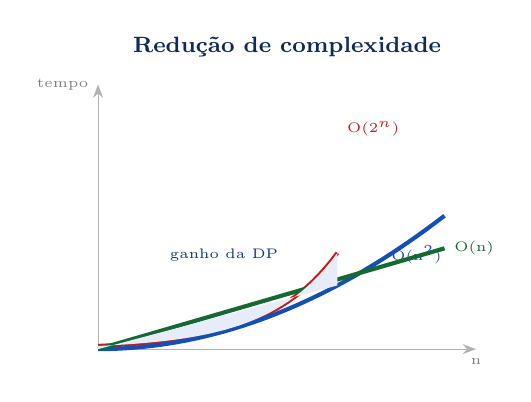
\begin{tikzpicture}[scale=0.80]
        \node[font=\bfseries\footnotesize,gemaBlue] at (3.0,4.8)
          {Redução de complexidade};
        % Eixos
        \draw[-{Stealth},gray!60,thin](0,0)--(6,0);
        \draw[-{Stealth},gray!60,thin](0,0)--(0,4.2);
        \node[font=\tiny,gray,below] at (6,0){n};
        \node[font=\tiny,gray,left] at (0,4.2){tempo};
        % Curva exponencial
        \draw[gemaRed,line width=1.5pt]
          plot[domain=0:3.8,samples=40]
          (\x, {min(3.8, 0.05*exp(\x*0.9))});
        \node[font=\tiny,gemaRed,right] at (3.8,3.5){O($2^n$)};
        % Curva polinomial
        \draw[dpBlue,line width=1.5pt]
          plot[domain=0:5.5,samples=40]
          (\x, {0.07*\x*\x});
        \node[font=\tiny,dpBlue,right] at (4.5,1.5){O(n$^2$)};
        % Curva linear
        \draw[gemaGreen!70!black,line width=1.5pt]
          (0,0)--(5.5,1.6);
        \node[font=\tiny,gemaGreen!70!black,right] at (5.5,1.6){O(n)};
        % Area de ganho
        \fill[dpBlue!10] (0,0)
          plot[domain=0:3.8,samples=40](\x,{min(3.8,0.05*exp(\x*0.9))})
          -- (3.8,0.07*3.8*3.8) -- (0,0);
        \node[font=\tiny,dpBlue!70!black] at (2.0,1.5){ganho da DP};
      \end{tikzpicture}
  \end{columns}
\end{frame}

% % ── RECEITA ─────────────────────────────────────────────────
% \begin{frame}{Como Pensar em DP --- Receita em 5 Passos}
%   \centering
%   \begin{adjustbox}{max totalsize={0.97\textwidth}{0.78\textheight},center}
%   \begin{tikzpicture}[scale=0.90]

%     \foreach \n/\x/\title/\desc/\col in {
%       1/1.4/{1. Identifique o objetivo}/{O que precisa ser maximizado,\\minimizado ou contado?}/dpBlue,
%       2/4.2/{2. Defina o estado}/{O que caracteriza um subproblema?\\dp[i], dp[i][j], ...}/dpTeal,
%       3/7.0/{3. Escreva a transição}/{Como combinar estados menores?\\dp[i] = função(dp[i-1], ...)}/gemaGreen,
%       4/9.8/{4. Defina os casos base}/{Quais estados voce conhece\\sem calcular?}/gemaOrange,
%       5/12.6/{5. Implemente e teste}/{Tabulação ou memoization?\\Verifique com exemplos!}/gemaPurple}{
%       \node[draw=\col,fill=\col!10,rounded corners=8pt,
%             minimum width=2.5cm,minimum height=3.0cm,
%             text width=2.3cm,align=center,
%             line width=0.9pt] at (\x,2.5){};
%       \node[draw=\col,fill=\col,circle,minimum size=9mm,
%             font=\bfseries\small,text=white] at (\x,4.2){\n};
%       \node[font=\bfseries\tiny,\col!80!black,align=center] at (\x,3.5){\title};
%       \node[font=\tiny,align=center] at (\x,2.3){\desc};
%     }

%     % Setas entre passos
%     \foreach \x in {2.7,5.5,8.3,11.1}{
%       \draw[-{Stealth},gray!50,line width=1pt](\x,2.5)--(\x+0.5,2.5);
%     }

%     % Exemplo abaixo
%     \node[draw=gemaBlue!30,fill=gemaBlue!5,rounded corners=4pt,
%           minimum width=13cm,text width=12.8cm,align=center,
%           font=\footnotesize] at (7.0,0.8)
%       {\textbf{Exemplo (Knapsack):}
%        Obj: max valor | Estado: dp[i][j] = max valor com i itens, cap. j |
%        Trans: max(nao pega, pega) | Base: dp[0][j]=0};

%   \end{tikzpicture}
%   \end{adjustbox}
% \end{frame}

% % ── COMO IDENTIFICAR NA OBI ─────────────────────────────────
% \begin{frame}{Como Identificar Problemas de DP na OBI?}
%   \begin{columns}[t]
%     \column{0.47\textwidth}
%       \begin{block}{Sinais de DP no enunciado}
%         \begin{itemize}\footnotesize
%           \item ``\textbf{maximo/minimo} de algo''
%           \item ``\textbf{número de formas} de...''
%           \item ``\textbf{existe} alguma combinação que...''
%           \item ``\textbf{particionamento} otimo''
%           \item Decisao sequêncial (etapas)
%           \item Subproblemas que se repetem
%           \item n $\leq$ 10$^3$ (sugere O(n$^2$) ou O(n$^3$))
%           \item Pares (n,W), (n,S): sugere 2D
%         \end{itemize}
%       \end{block}
%       \vspace{0.10cm}
%       \begin{tcolorbox}[caixaLaranja,title={Palavras-chave tipicas}]
%         \footnotesize
%         ``subsequência'', ``subconjunto'', ``mochila'',
%         ``caminho'', ``partição'', ``corte'',
%         ``seleção de itens'', ``planejamento''
%       \end{tcolorbox}
%     \column{0.50\textwidth}
%       \begin{tcolorbox}[caixaVermelho,title={Quando NAO usar DP}]
%         \begin{itemize}\footnotesize
%           \item Problema tem \textbf{greedy choice property} clara\\
%                 $\to$ Use Guloso (mais simples!)
%           \item Subproblemas \textbf{nao se repetem}\\
%                 $\to$ Divisao e Conquista
%           \item Sem \textbf{subestrutura otima}\\
%                 $\to$ Nem guloso nem DP
%           \item $n > 10^5$ e DP seria O(n$^2$)\\
%                 $\to$ Busque estrutura de dados ou guloso
%         \end{itemize}
%       \end{tcolorbox}
%       \vspace{0.10cm}
%       \begin{tcolorbox}[caixaDP,title={Teste rápido}]
%         \footnotesize
%         \textbf{1.} Consigo definir dp[i] claramente?\\
%         \textbf{2.} Consigo calcular dp[i] a partir de dp[j<i]?\\
%         \textbf{3.} Resolvo o problema menor primeiro?\\[3pt]
%         Se sim para os 3: provavelmente e DP!
%       \end{tcolorbox}
%   \end{columns}
% \end{frame}

% ── ERROS COMUNS ────────────────────────────────────────────
\begin{frame}{Erros Comuns em DP}
  \centering
  \begin{adjustbox}{max totalsize={0.96\textwidth}{0.78\textheight},center}
  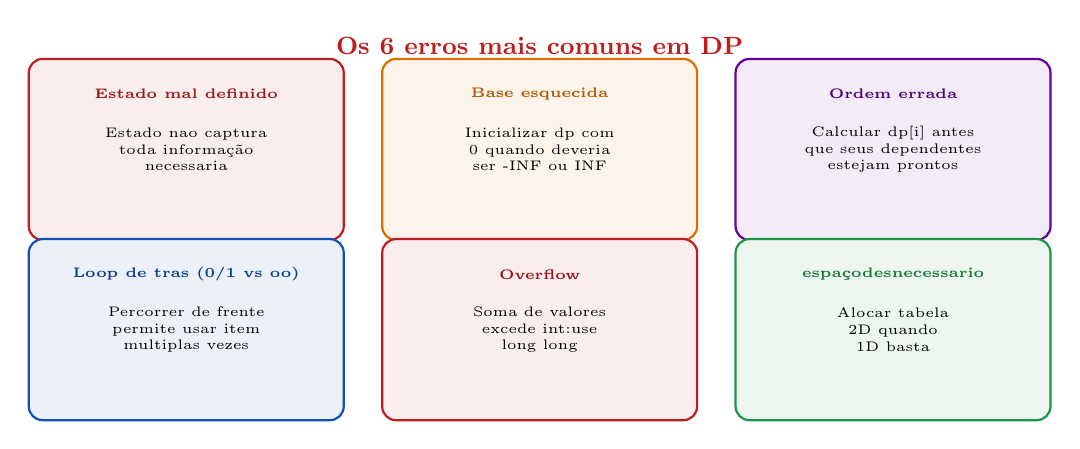
\begin{tikzpicture}[scale=0.88]

    \node[font=\bfseries\small,gemaRed] at (7.0,5.3)
      {Os 6 erros mais comuns em DP};

    \foreach \x/\y/\title/\desc/\cor in {
      1.9/3.8/{Estado mal definido}/{Estado nao captura\\toda informação\\necessaria}/gemaRed,
      7.0/3.8/{Base esquecida}/{Inicializar dp com\\0 quando deveria\\ser -INF ou INF}/gemaOrange,
      12.1/3.8/{Ordem errada}/{Calcular dp[i] antes\\que seus dependentes\\estejam prontos}/gemaPurple,
      1.9/1.2/{Loop de tras (0/1 vs oo)}/{Percorrer de frente\\permite usar item\\multiplas vezes}/dpBlue,
      7.0/1.2/{Overflow}/{Soma de valores\\excede int:use\\long long}/gemaRed,
      12.1/1.2/{espaçodesnecessario}/{Alocar tabela\\2D quando\\1D basta}/gemaGreen}{
      \node[draw=\cor,fill=\cor!8,rounded corners=5pt,
            minimum width=4.0cm,minimum height=2.3cm,
            text width=3.6cm,align=center,
            font=\tiny,line width=0.8pt] at (\x,\y){};
      \node[font=\bfseries\tiny,\cor!80!black,align=center] at (\x,\y+0.8){\title};
      \node[font=\tiny,align=center] at (\x,\y){\desc};
    }

  \end{tikzpicture}
  \end{adjustbox}
\end{frame}

% ── COMPARAÇÃO GULOSO VS DP ─────────────────────────────────
\begin{frame}[shrink=2]{Comparação: Guloso vs Programação Dinâmica}
  \begin{tcolorbox}[caixaAzul,title={Quando usar cada paradigma?}]
    \centering\footnotesize
    \begin{tabular}{lcc}
      \toprule
      \textbf{Criterio} & \textbf{Guloso} & \textbf{Prog. Dinamica}\\
      \midrule
      Corretude          & Se provar     & Sempre (se modelar certo)\\
      Complexidade       & O(n log n)    & O(n$\cdot$k) polinomial\\
      Implementação      & Simples       & Media\\
      Precisa provar?    & Sim           & Nao (mas ajuda)\\
      Revisa decisoes?   & Nao           & Sim (implicitamente)\\
      Subproblemas rep.? & Nao           & Sim (essencial)\\
      Mochila 0/1        & Nao funciona  & Funciona\\
      Mochila fracionaria& Funciona      & Funciona (desnecessario)\\
      Fibonacci          & Nao se aplica & Funciona perfeitamente\\
      \bottomrule
    \end{tabular}
  \end{tcolorbox}
  \vspace{0.10cm}
  \begin{columns}[t]
    \column{0.31\textwidth}
      \begin{tcolorbox}[caixaDourada,title={Guloso}]
        \footnotesize
        Decisao local otima.\\
        Sem revisitar.\\
        Prove o exchange argument.
      \end{tcolorbox}
    \column{0.31\textwidth}
      \begin{tcolorbox}[caixaDP,title={Programação Dinâmica}]
        \footnotesize
        Subproblemas sobrepostos.\\
        Subestrutura otima.\\
        Memoriza tudo.
      \end{tcolorbox}
    \column{0.31\textwidth}
      \begin{tcolorbox}[caixaVermelho,title={Forca Bruta}]
        \footnotesize
        Nenhuma das duas.\\
        Pequenos n.\\
        Util para testar solucoes.
      \end{tcolorbox}
  \end{columns}
\end{frame}

% % ── PROBLEMAS PARA PRATICAR ─────────────────────────────────
% \begin{frame}{Problemas Classicos para Praticar}
%   \begin{columns}[t]
%     \column{0.48\textwidth}
%       \begin{tcolorbox}[caixaVerde,title={Iniciante}]
%         \begin{itemize}\footnotesize
%           \item \textbf{CSES 1633} --- Dice Combinations (somar de 1 a 6)
%           \item \textbf{CSES 1634} --- Minimizing Coins (troco DP)
%           \item \textbf{CSES 1635} --- Coin Combinations I (contar formas)
%           \item \textbf{CF 189A} --- Cut Ribbon
%           \item \textbf{OBI} --- Subconjunto de soma S
%         \end{itemize}
%       \end{tcolorbox}
%       \vspace{0.08cm}
%       \begin{tcolorbox}[caixaDP,title={Intermediario}]
%         \begin{itemize}\footnotesize
%           \item \textbf{CSES 1745} --- Money Sums (Subset Sum)
%           \item \textbf{CSES 1158} --- Book Shop (Knapsack)
%           \item \textbf{CF 455A} --- Boredom
%           \item \textbf{CF 837D} --- Round Subset
%           \item \textbf{LC 322} --- Coin Change
%         \end{itemize}
%       \end{tcolorbox}
%     \column{0.48\textwidth}
%       \begin{tcolorbox}[caixaRoxa,title={Avancado}]
%         \begin{itemize}\footnotesize
%           \item \textbf{CSES 1639} --- Edit Distance (LCS/LCS)
%           \item \textbf{CSES 1140} --- Longest Increasing Subseq.
%           \item \textbf{CF 1513C} --- Add One
%           \item \textbf{CF 368B} --- Sereja and Suffixes
%           \item \textbf{LC 1143} --- Longest Common Subsequence
%         \end{itemize}
%       \end{tcolorbox}
%       \vspace{0.08cm}
%       \begin{tcolorbox}[caixaAmarelo,title={Roteiro de estudo}]
%         \footnotesize
%         \begin{enumerate}\footnotesize
%           \item Resolva Fibonacci nos 3 modos
%           \item Implemente Knapsack do zero
%           \item Resolva 5 problemas do CSES DP
%           \item Identifique o estado em 3 CF novos
%           \item Leia editorial de 1 problema avancado
%         \end{enumerate}
%       \end{tcolorbox}
%   \end{columns}
% \end{frame}

% ── RESUMO ──────────────────────────────────────────────────
\begin{frame}[shrink=2]{Resumo Geral --- Programação Dinâmica}
  \begin{columns}[t]
    \column{0.31\textwidth}
      \begin{block}{O que e?}
        \begin{itemize}\footnotesize
          \item recursão + Memorização
          \item Resolve cada subprob. 1x
          \item Exige subprob. sobrepostos
          \item E subestrutura otima
        \end{itemize}
      \end{block}
      \vspace{0.08cm}
      \begin{block}{4 Pilares}
        \begin{itemize}\footnotesize
          \item \textbf{Estado:} o que guardar
          \item \textbf{Transição:} a fórmula
          \item \textbf{Base:} casos triviais
          \item \textbf{Ordem:} bottom-up
        \end{itemize}
      \end{block}
    \column{0.31\textwidth}
      \begin{block}{Problemas vistos}
        \begin{itemize}\footnotesize
          \item Fibonacci: O(n)/O(1)
          \item Knapsack 0/1: O(n$\cdot$W)
          \item Subset Sum: O(n$\cdot$S)
        \end{itemize}
      \end{block}
      \vspace{0.08cm}
      \begin{block}{Abordagens}
        \begin{itemize}\footnotesize
          \item Tabulação: bottom-up (preferir)
          \item Memoization: top-down (protitipar)
          \item Otimização 1D: de tras para frente
        \end{itemize}
      \end{block}
    \column{0.31\textwidth}
      \begin{tcolorbox}[caixaDP,title={Receita}]
        \footnotesize
        \textbf{1.} Qual o objetivo?\\[2pt]
        \textbf{2.} Defina dp[estado]\\[2pt]
        \textbf{3.} Escreva transição\\[2pt]
        \textbf{4.} Defina casos base\\[2pt]
        \textbf{5.} Implemente e teste
      \end{tcolorbox}
      \vspace{0.08cm}
      \begin{tcolorbox}[caixaVermelho,title={Erro fatal}]
        \footnotesize
        \textbf{Estado mal definido} = toda a
        solução esta errada.\\[3pt]
        Pense bem no estado antes de codar!
      \end{tcolorbox}
  \end{columns}
\end{frame}

% ── SLIDE FINAL ─────────────────────────────────────────────
{
\setbeamertemplate{footline}{}
\begin{frame}[noframenumbering]
  \centering\vspace{0.08cm}
  \begin{columns}[c]
    \column{0.28\textwidth}
      \centering
\includegraphics[width=0.65\linewidth]{logo.png}
    \column{0.42\textwidth}
      \centering
      {\large\color{gemaBlue}\bfseries Bons estudos\\e boa prova!}\par
      \vspace{0.10cm}
      {\small\color{gemaCyan} GEMA --- Maratonas de Programação}\par
      \vspace{0.10cm}
    \column{0.28\textwidth}
      \centering
\includegraphics[width=0.65\linewidth]{logo_obi.png}
  \end{columns}

\end{frame}
}

\end{document}